\begin{frame}{Rete VDSR}
    \begin{block}{Rete VDSR}
        Per cercare di superare le limitazioni della rete ispirata al paper SRCNN 2014
        ci si è ispirati al paper \textbf{Very Deep Super Resolution} del 2015.

        Le uniche cose che sono state modificate sono:
        \begin{itemize}
            \item Architettura della rete
            \item Funzione di loss L1 invece di MSE
            \item Batch normalization tra i layer di convoluzione
            \item Aggiunta del residual learning
        \end{itemize}
    \end{block}
\end{frame}

\begin{frame}{Architettura rete VDSR}
    \begin{block}{Rete VDSR}
    \begin{itemize}
            \item Il paper utilizza circa 20 layer di convoluzione
            \item È stato deciso di utilizzarne solo 7 per praticità
            \item Ogni layer ha 64 canali in output
    \end{itemize}
    \end{block}


    \begin{figure}
        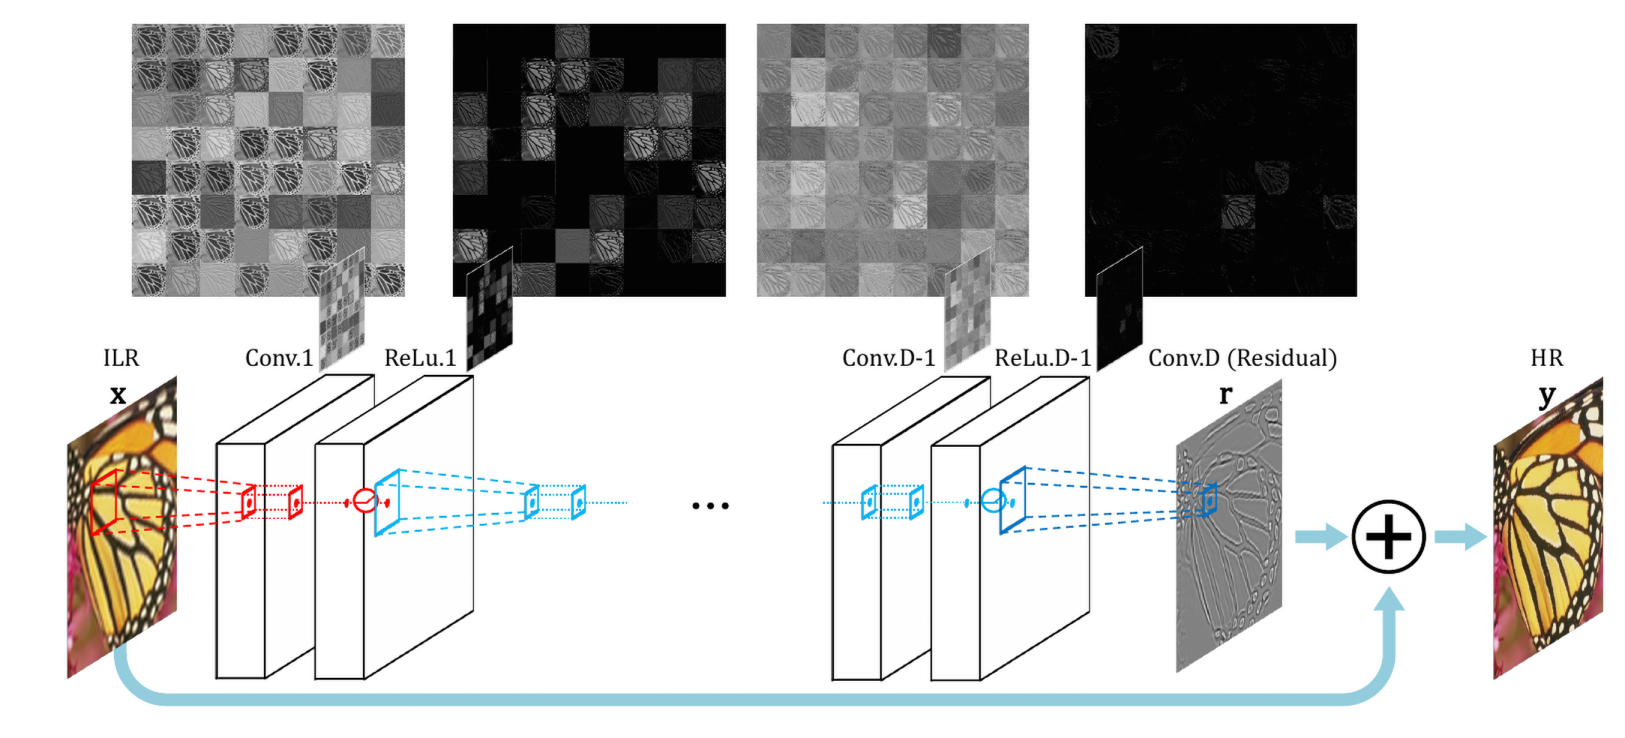
\includegraphics[width=0.8\textwidth]{figures/architettura_VDSR.png}
    \end{figure}
\end{frame}

\begin{frame}{Risultati con rete VDSR}
    \begin{block}{Risultati}

    Con questa architettura è stato possibile superare un'istanza del test set.

    \end{block}

    \begin{figure}
        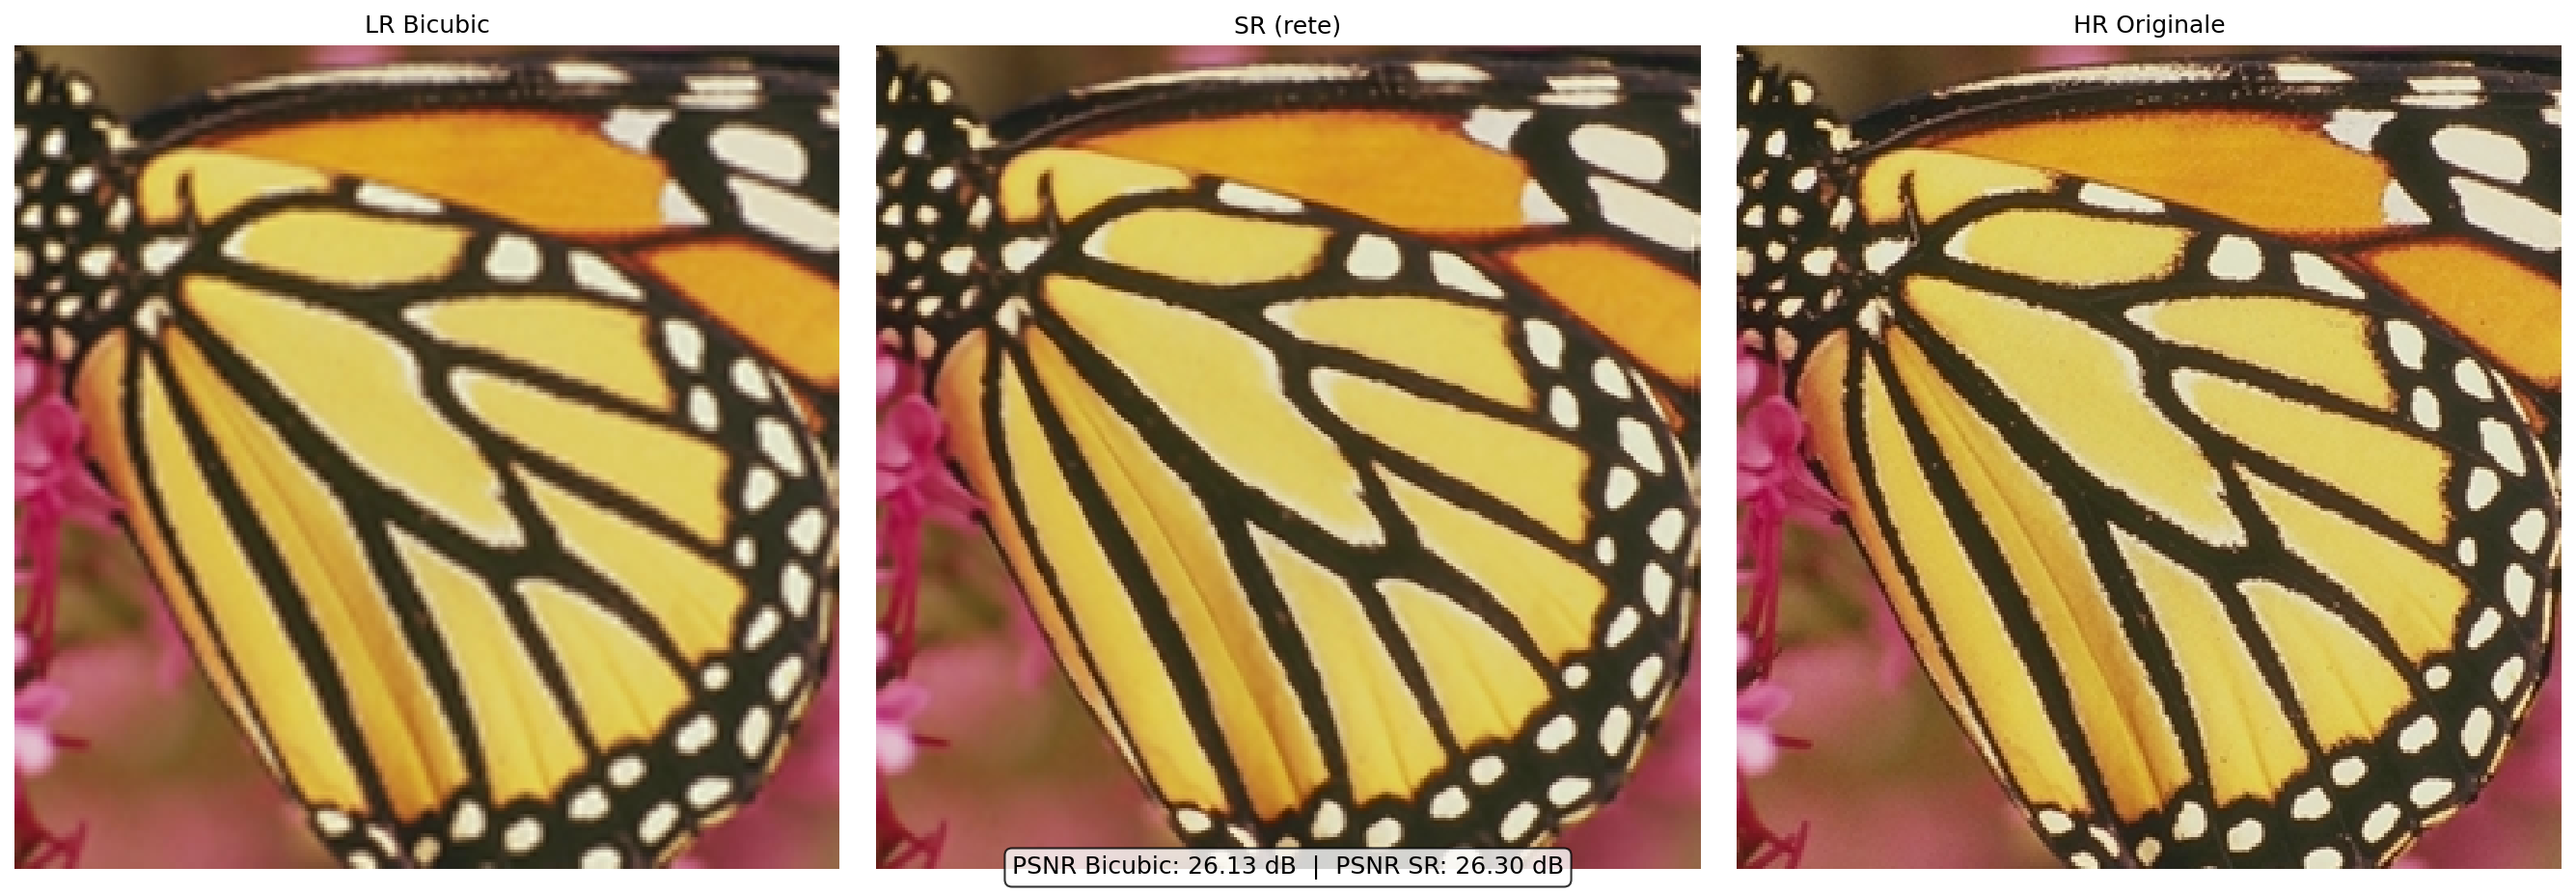
\includegraphics[width=1\textwidth]{figures/risultato_migliore.png}
    \end{figure}
\end{frame}